\documentclass[12pt,a4paper]{article}

\usepackage[utf8]{inputenc}

\usepackage[width=200mm,height=290mm,centering]{geometry}

% \usepackage{mathptmx}
% \usepackage{palatino}

%\usepackage{chancery}
%\usepackage{antiqua}
%\usepackage{aboensis}
\usepackage{gfsartemisia-euler}
\usepackage[T1]{fontenc}

% \usepackage{fontspec}
% \setmainfont{QTChanceryType}

\usepackage{graphicx}
\usepackage[table]{xcolor}
\usepackage{tikz}
\usepackage[hidelinks]{hyperref}

\pagestyle{empty}

\newcommand{\logo}{\makebox[56mm][c]{\rule{0mm}{66mm}\raisebox{12mm}{
\includegraphics[width=48mm]{logo/aldc-4couleurs-3.pdf}}}}

%\pagecolor{yellow!5}

\begin{document}
%\sffamily

\vspace*{-20mm}\hspace*{-15mm}
\begin{tikzpicture}(20,7)
\shade[right color=black, left color=violet!60!white] (-8,0) rectangle (3.05,7);
\shade[left color=black, right color=violet!60!white] (3,0) rectangle (14,7);
%\node at (-4,3){\logo};
\node at (3,3){\logo};
%\node at (10,3){\logo};
\end{tikzpicture}

% \begin{minipage}{1.0\linewidth}
% \colorbox{blue!50}{
\includegraphics[width=50mm]{images/logo.png}}
% \end{minipage}

%\vfill

\begin{center}

\bfseries
\color{orange!75!black}

\LARGE

Rentrée 2025-2026

 Reprises des cours le mercredi 10 septembre

\vfill

% \href{https://alevisdanse.github.io}{
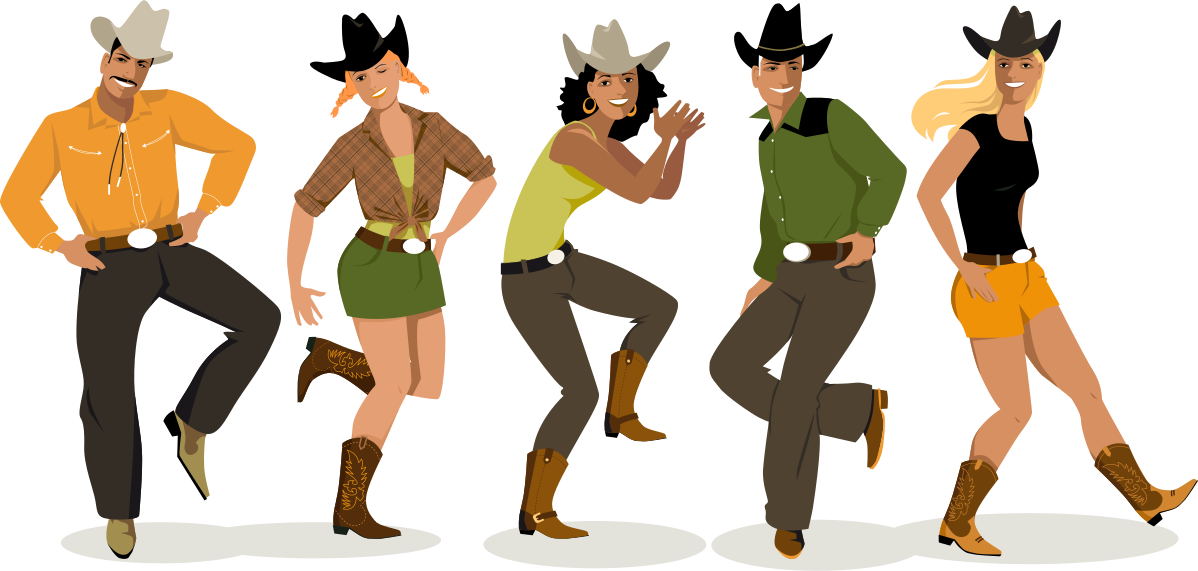
\includegraphics[width=0.9\textwidth]{groupe.pdf}
%}

\color{green!50!black}%
Une Ambiance Conviviale à Lévis-Saint-Nom

\color{blue!50!black}%
VENEZ DANSER \& VOUS DÉTENDRE

\vfill

\large
\setlength\arrayrulewidth{2pt}
\arrayrulecolor{brown}
\color{brown!50!black}
\begin{tabular}{|c|c|c|}
  \hline
  \rowcolor{orange!10}
  Cours débutant & mercredi & de 20h à 21h \\
  \hline
  \rowcolor{orange!20}
  Cours novice & mercredi & de 21h à 22h \\
  \hline
  \rowcolor{orange!30}
  Cours intermédiaire & jeudi & de 20h15 à 21h15 \\
  \hline
  \rowcolor{green!20}%
  \color{green!25!black}%
  Country catalan ou partner & jeudi & de 21h15 à 22h15 \\
  \rowcolor{green!20}%
  \color{green!25!black}%
  (en alternance) &  &  \\
  \hline
\end{tabular}
\vfill

\Large

\color{red!70!black}%
Cours d'essai GRATUIT en septembre

\vfill

\href{https://alevisdanse.github.io}{\raisebox{-20mm}{\includegraphics[width=40mm]{images/qr-code.pdf}}}
\qquad
\begin{minipage}[c]{0.45\textwidth}
  \Huge\color{black!50!blue}  \href{https://alevisdanse.github.io}{Plus d'information sur notre page web \\
    $\longleftarrow$}
\end{minipage}

\end{center}

\end{document}














\begin{center}
\href{https://alevisdanse.github.io}{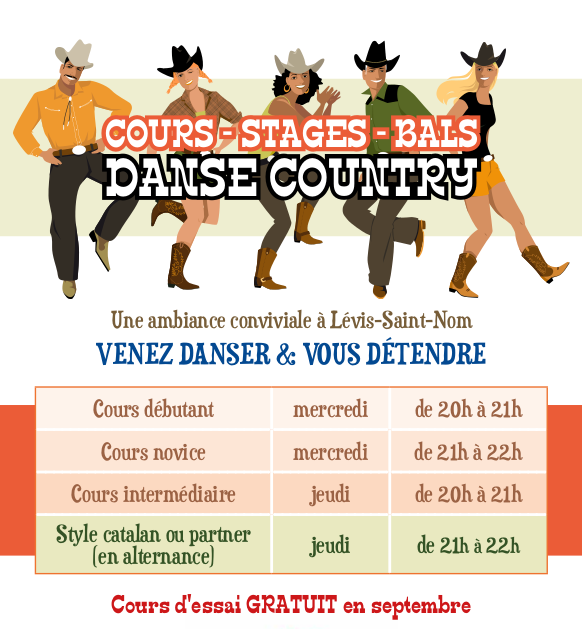
\includegraphics{images/flyerLCLD.png}}

\vfill\vfill

\href{https://alevisdanse.github.io}{\raisebox{-20mm}{\includegraphics[width=40mm]{images/qr-code.pdf}}}
\qquad
\begin{minipage}[c]{0.37\textwidth}
\Huge\color{black!50!blue}  \href{https://alevisdanse.github.io}{Plus d'information sur notre page web $\longleftarrow$}
\end{minipage}

\end{center}

\end{document}
